\documentclass[10pt, a4paper]{article}

% --- Packages ---
\usepackage[utf8]{inputenc}
\usepackage[T1]{fontenc}
\usepackage[margin=2cm]{geometry} % Modern, slightly tighter margins
\usepackage{xcolor}
\usepackage{titlesec}
\usepackage{multicol} % For the 2-column magazine feel
\usepackage{enumitem}
\usepackage{graphicx}
\usepackage{abstract}
\usepackage{microtype} % Better kerning
\usepackage{fontspec} % Requires XeLaTeX/LuaLaTeX
\usepackage{amsmath}
\usepackage{amssymb}
\usepackage{tikz}
\usepackage{float}
\usepackage{graphicx}

\graphicspath{ {./images/} } % This tells LaTeX to look in the 'images' folder

\usetikzlibrary{shapes,arrows,positioning}

% --- Aesthetic Setup ---
\definecolor{collectiveBlue}{HTML}{0056b3}

% Custom Fonts (Assuming standard Ubuntu fonts, or swap for your favs)
\newfontfamily\headerfont{FreeSans} 
\setmainfont{FreeSerif}

% Commands for convenience
\newcommand{\magazineRule}{
    \nointerlineskip \vspace{0.5em}
    \noindent\rule{\textwidth}{1.2pt}
    \vspace{0.5em}
}

% Header Styling
\titleformat{\section}{\large\headerfont\bfseries\color{collectiveBlue}}{}{0em}{\MakeUppercase}
\titleformat{\subsection}{\normalsize\headerfont\bfseries}{}{0em}{}

% --- Document Info ---
\title{
    {\headerfont\Huge \textbf{Collective}} \\
    \vspace{0.5em}
    {\large \textit{A Ubiquitous Computational Model for a Post-Market Collaborative Society}}
}
\author{J.C. Novais Raffaine \\ \small \texttt{dev.epensieve.com}}
\date{\today}

% --- The Document ---
\begin{document}

\maketitle

% --- Abstract (Single Column) ---
\begin{abstract}
% File: sections/00_abstract.tex

\noindent This paper proposes \textbf{Collective}, a decentralized architecture for social coordination designed to supersede the competitive, individualistic logic of traditional market economies. By conceptualizing the economy as a form of \textit{ubiquitous computation}—a distributed virtual machine for the satisfaction of community demand—we move beyond the constraints of private ownership and wage-based labor. 

The system is architected as a federated mesh of recursive \textbf{Service Nodes}, which utilize a Work Breakdown Structure (WBS) modeled via Business Process Model and Notation (BPMN) to map community needs to executable tasks. We introduce a dual-token metabolic model: \textit{Value}, a liquid credit for lifestyle construction that facilitates unbounded negative balances for social security; and \textit{Tokens}, a non-transferable reputation metric earned through labor and required for node-level governance. 

The structural integrity of the mesh is maintained by \textbf{Societies}, specialized nodes that represent the legal and territorial logic of the community, governing resource stewardship and member rights. Central to the model is the \textbf{Common Fund}, which mediates the "lease" of external resources to allow Collective cells to coexist with and eventually "leach" the legacy market. Through the integration of \textbf{Bodies of Knowledge} for skill verification and \textbf{Prospecting Engines} for demand forecasting, Collective provides a scalable framework for a post-scarcity metabolism. Ultimately, the system transforms the daily actions of human interaction into a self-organizing protocol, enabling the phased transition toward a society where contribution is the sole investment and utility is the primary output.
\end{abstract}

\vspace{2em}
\magazineRule % Horizontal rule for style

% --- Body (Double Column) ---
\begin{multicols}{2}

% File: sections/01_intro.tex

\section{Introduction}

The contemporary global economy is predicated on a 19th-century interpretation of market dynamics: a reactive, competitive struggle for resource dominance. While this model facilitated rapid industrialization, it has proven increasingly ineffective at addressing the complexities of a hyper-connected, resource-constrained world. The current market-based system suffers from systemic "information entropy," where the lack of transparent, real-time demand signaling leads to profound inefficiencies.

\subsection{The Inefficiency of Market Opaque-ness}
Current resource handling is largely speculative. In the legacy market, production precedes demand, driven by the necessity of capturing market share and profit margins. This results in staggering waste: globally, nearly 1.3 billion tons of food are wasted annually \cite{fao2021}, while "just-in-case" inventory models lead to massive energy expenditure for products that may never reach a consumer. These are not mere logistical errors; they are structural failures of a system that treats information as a proprietary secret rather than a shared utility.

\subsection{Ineffectiveness in Meeting Human Demand}
Furthermore, the market is frequently ineffective at meeting actual human demand. By prioritizing "effective demand"—the ability to pay—over "human demand," the system creates artificial scarcity in essential sectors like housing and healthcare while over-allocating resources to high-margin, low-utility commodities. This mismatch is exacerbated by the "bullwhip effect," where small fluctuations in consumer behavior cause amplified oscillations in supply chains, leading to boom-bust cycles that destabilize entire communities.

\subsection{The Information Gap: The Bullwhip Effect}
The aforementioned speculative nature of production is worsened by the "bullwhip effect" \cite{lee1997bullwhip}. This phenomenon occurs when a lack of transparent, ubiquitous data causes slight changes in consumer demand to be amplified as they move up the supply chain. The result is a chaotic cycle of over-manufacturing followed by massive liquidations, wasting both natural resources and human hours on products the community never actually demanded.

\subsection{Exacerbated Inequality and Poverty}
The legacy model’s reliance on capital accumulation inevitably leads to extreme wealth concentration \cite{oxfam2024}. As of the early 21st century, the world’s wealthiest 1\% own nearly half of all global household wealth, while billions remain in "working poverty"—a state where labor is performed but the resulting value is captured by capital owners rather than the laborers themselves. This systemic extraction is not just a social crisis but a computational one: it represents a massive "deadweight loss" where human potential is sidelined because it lacks the legacy currency to signal its needs.

\subsection{The Collective Paradigm}
\textbf{Collective} introduces a shift from reactive speculation to proactive computation. By utilizing a transparent and explicit model for value generation, the architecture ensures that every task fulfilled and every resource consumed is mapped directly to a verified community demand. 

In the sections that follow, we outline the technical and social pillars of this transition. Section 2 presents the overall Architecture and the Taxonomy of a Collective Cell. Section 3 details the \textbf{Service Node Modeler} and the usage of BPMN as the source code of production. Section 4 explores the \textbf{Token Metabolism}, explaining how we decouple survival from governance. Section 5 introduces the \textbf{Societies} and the \textbf{Common Fund}, providing the legal and financial framework for "leaching" the old system. Finally, we discuss the federated mesh architecture that allows Collective to scale from micro-instances into a global, ubiquitous infrastructure.

\section{System Taxonomy: Agents and Architecture}

Before detailing the computational processes of Collective, we must define the primary entities that inhabit and sustain the mesh. Unlike the rigid hierarchies of the legacy market, roles in Collective are fluid, determined by current activity rather than permanent employment status.

\subsection{Community Members (The Workers)}
The heart of the Collective is the \textbf{Community Member}, referred to functionally as the \textbf{Worker} during task execution. Members are the sole "processors" of the system. 
\begin{itemize}[leftmargin=*]
    \item \textbf{Sovereignty:} Members own their data and move freely between different Service Nodes and geographic instances.
    \item \textbf{Identity:} A Member's identity is tied to their global "Body of Knowledge" certifications and their accumulated Value balance.
\end{itemize}

\subsection{Service Nodes and Specialized Pillars}
The architecture is composed of recursive, specialized entities that provide the "Operating System" services:
\begin{enumerate}
    \item \textbf{Service Nodes:} The primary units of production (e.g., an Eco-Village bakery).
    \item \textbf{Bodies of Knowledge (BoK):} The educational kernel; they define what a Task is and verify if a Member possesses the required Skill.
    \item \textbf{Societies:} The legal and territorial layer; they govern the physical "Lease" of the land and protect member rights.
    \item \textbf{The Common Fund:} The metabolic gateway; it manages external procurement and internal liquidity.
\end{enumerate}

\subsection{Active Agents: Designers and Prospectors}
While every member is a Worker, some choose to act as \textbf{Service Designers} (the architects of the WBS) or \textbf{Demand Prospectors} (the sensory scouts identifying community needs). These roles allow the mesh to proactively evolve its production logic.

\section{The Service Node Modeler: The Social IDE}

The transition from an opaque, speculative market to an explicit, computational economy requires a specialized development environment. We term this the \textbf{Service Node Modeler}. Its purpose is to allow active agents—Designers and Workers—to model, simulate, and instantiate the Work Breakdown Structure (WBS) that governs community production.

\subsection{BPMN as Executable Logic}
Collective utilizes an extended version of \textit{Business Process Model and Notation} (BPMN) as its primary descriptive language. In this paradigm, a process diagram is not a static documentation of a workflow; it is the executable "source code" of the Service Node. 

When a Designer maps a process, they define:
\begin{itemize}[leftmargin=*]
    \item \textbf{Data Objects:} The Resources (internal or external) required for execution.
    \item \textbf{Service Tasks:} The specific units of labor defined by the Body of Knowledge (BoK).
    \item \textbf{Sequence Flows:} The logical dependencies and prerequisites for task activation.
\end{itemize}

\subsection{Property-Driven Reactivity}
Each Service Node is a state machine. The Modeler allows for the definition of "Environment Properties" such as \textit{Stocking Levels}, \textit{Risk Thresholds}, and \textit{Demand Urgency}. 

For example, a "Food Distribution Node" may have a logic gate: \textit{IF Stock < 15\% THEN Escalate Logistics Tasks to CRITICAL Priority}. This allows the ubiquitous system to react to physical reality in real-time without the lag of human administrative intervention or market price signals.

\subsection{Predictive Readiness and Availability Tasks}
A significant challenge in on-demand services is the "cold-start" problem—ensuring human presence before the demand event occurs. The Modeler addresses this via \textbf{Availability Tasks}. These are "Warm Standby" processes where Workers are compensated for their presence within the Node environment. By analyzing data from the \textbf{Prospecting Engine}, the Node can pre-scale its "Availability Tasks" to ensure that, for instance, a medical professional or a chef is checked-in and ready the moment a demand event is triggered.
\subsection{Governance via Stored Reputation}
The Modeler is not merely a technical tool but a political one. As Workers fulfill tasks within a specific Node, they accumulate non-transferable \textit{Reputation Tokens}. These tokens represent the "Skin in the Game" required to influence the Node’s operational logic. To refine a WBS or alter the environment properties, Workers must "spend" or stake their tokens within the Modeler. This ensure that the architectural evolution of the Node is directed by those with the highest operational context, creating a functional meritocracy that prevents "governance spam" from unverified actors.

\subsection{Inter-Node Dependencies}
A Service Node does not exist in a vacuum; its WBS is interconnected with the specialized "System Nodes" of the mesh:
\begin{itemize}[leftmargin=*]
    \item \textbf{BoK Integration:} The Modeler pulls standardized "Task Classes" from the Bodies of Knowledge, which also handle the asynchronous verification of Worker Skills.
    \item \textbf{Common Fund Mediation:} When a process requires "External Resources" (those not produced within the Collective), the Modeler triggers a request to the Common Fund to manage the legacy-market lease.
    \item \textbf{Societal Anchorage:} Every Service Node is anchored to a physical or legal jurisdiction via the \textbf{Societies}, which provide the territorial permissions and rights framework necessary for execution.
\end{itemize}

\subsection{The Service Node Lifecycle}
The trajectory of a Node follows a standardized path within the Modeler: \textit{Prospecting} (identifying demand), \textit{Design} (modeling the initial WBS), \textit{Founding/Ratification} (initial resource and worker commitment), and \textit{Operation} (continuous task execution and refinement). This lifecycle allows the Collective to remain fluid—Nodes that no longer satisfy a community demand naturally hibernate or dissolve, releasing resources back to the Common Fund. (The specific mechanics of bootstrapping new cells and Node maturation are explored in Section 6).

\begin{figure*}
\centering
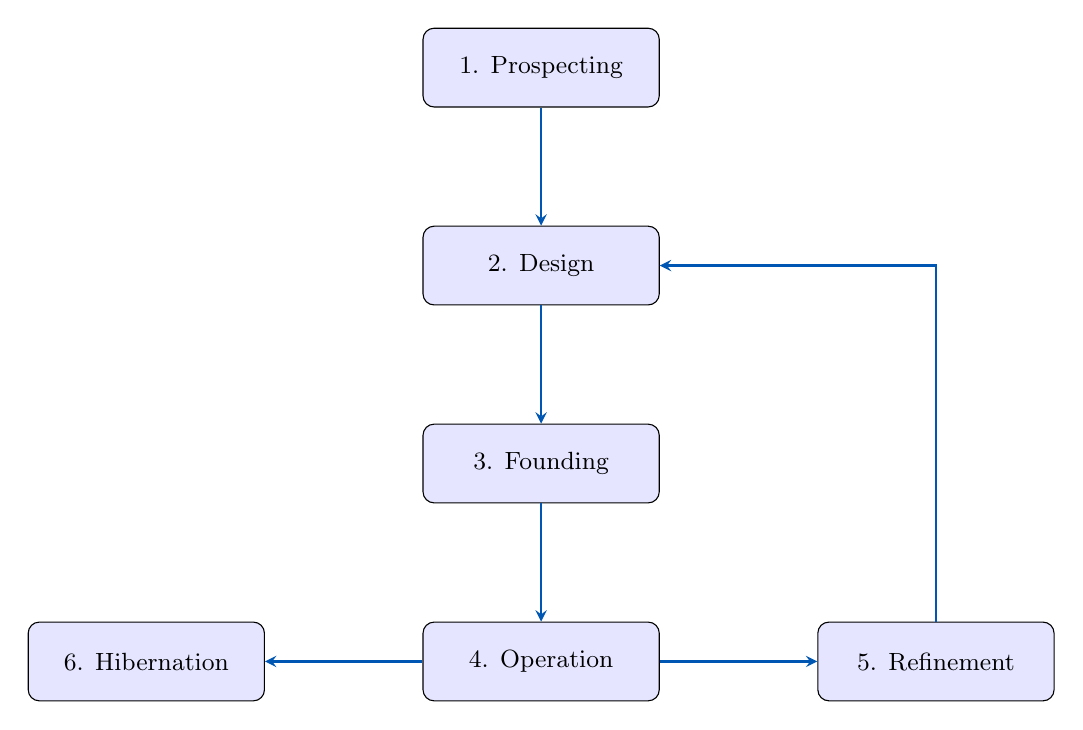
\begin{tikzpicture}[
    node distance = 1.5cm and 1cm,
    state/.style = {rectangle, draw, fill=blue!10, rounded corners, font=\headerfont\small, text centered, minimum width=3cm, minimum height=1cm},
    arrow/.style = {->, >=stealth, thick, color=collectiveBlue}
]

% Nodes
\node [state] (prospect) {1. Prospecting };%\\ \scriptsize (Demand Signal)};
\node [state, below=of prospect] (design) {2. Design }; %\\ \scriptsize (WBS/BPMN Modeling)};
\node [state, below=of design] (founding) {3. Founding }; %\\ \scriptsize (Ratification \& Lease)};
\node [state, below=of founding] (operate) {4. Operation };%\\ \scriptsize (Task Execution)};
\node [state, right=2cm of operate] (refine) {5. Refinement };%\\ \scriptsize (Token Spending)};
\node [state, left=2cm of operate] (hibernate) {6. Hibernation };%\\ \scriptsize (Resource Release)};

% Arrows
\draw [arrow] (prospect) -- (design);
\draw [arrow] (design) -- (founding);
\draw [arrow] (founding) -- (operate);
\draw [arrow] (operate.east) -- ++(0.5,0) |- (refine.west);
\draw [arrow] (refine.north) |- (design.east);
\draw [arrow] (operate.west) -- (hibernate.east);

\end{tikzpicture}
\caption{The recursive lifecycle of a Service Node within the Collective.}
\end{figure*}


\section{The Token Metabolism: Value and Governance}

The Collective operates on a dual-token metabolic system designed to decouple an individual's right to exist from their influence over social production. By separating "Value" from "Governance Tokens," the system prevents the accumulation of capital from translating into the accumulation of power.

\subsection{Value: The Signal for Lifestyle Construction}
\textit{Value} is a liquid, measurable credit earned through the fulfillment of Tasks within any Service Node. It represents the Member's claim on the community's collective output. 
\begin{itemize}[leftmargin=*]
    \item \textbf{Metabolic Flow:} Value is issued by a Node upon task completion and is "consumed" when a Member utilizes a service (e.g., lodging or nourishment).
    \item \textbf{The Unbounded Negative Balance:} Unlike legacy debt, a negative Value balance does not carry interest or punitive measures. It is a functional signal of "invested potential." This allows the system to support Members during education, illness, or the bootstrapping of new, high-resource Service Nodes. 
\end{itemize}

\subsection{Reputation Tokens: The Skin-in-the-Game Metric}
While Value is global and liquid, \textit{Tokens} are local and non-transferable. They represent a Member's verified contribution to a specific Service Node.
\begin{itemize}[leftmargin=*]
    \item \textbf{Earning Logic:} Tokens are granted alongside Value but are partitioned by the Node of origin. A Member may be "Value-wealthy" but "Token-poor" in a specific domain if they have not contributed labor to it.
    \item \textbf{Spend-to-Change Governance:} Influence is a consumable resource. To propose alterations to a Node's BPMN logic or to ratify a new Resource lease, Members must stake or spend their Tokens. This ensures that only those with a history of operational success (Reputation) can steer the Node's future.
\end{itemize}

\subsection{Decoupling Survival from Influence}
This dual-token architecture solves a fundamental failure of the market: the "Plutocratic Leak." In the legacy system, those with the most currency (Value) automatically gain the most voting power (Tokens). In Collective, these two vectors are orthogonal. A Member may consume at a high level due to past contributions (High Value) but lose their ability to govern a Node if they cease to actively participate in its tasks (Depleting Tokens). This creates a dynamic, labor-based meritocracy that remains perpetually responsive to the active community.

\subsection{The Cost of Change: Governance as Resource Allocation}
The "Spend-to-Change" mechanic is governed by an algorithmic cost function within the Service Node Modeler. This ensures that systemic changes are commensurate with the effort required to implement them and the risk they pose to the Node's stability.

\subsubsection{The Complexity Variable}
The Token cost for an alteration is not arbitrary; it is a function of the BPMN model’s \textit{Structural Complexity Index} (SCI). Adding a simple "Informational Task" carries a lower cost than altering a "Resource Gateway" or a "Critical Path" logic gate. 
\[ Cost_{Tokens} = f( \Delta \text{Tasks}, \sigma \text{Risk}, \Omega \text{Dependency} ) \]
Where $\Delta$ represents the volume of change, $\sigma$ the risk threshold of the affected nodes, and $\Omega$ the number of downstream dependencies in the federated mesh.

\subsubsection{Consumable vs. Staked Influence}
To provide flexibility in governance, the system distinguishes between two modes of Token usage:
\begin{itemize}[leftmargin=*]
    \item \textbf{Consumable Spend:} For minor tactical adjustments (e.g., shifting task priorities), Tokens are "consumed" (burned), requiring the Member to return to the Work to regain influence.
    \item \textbf{Staked Commitment:} For strategic structural changes (e.g., merging Nodes or changing the Core WBS), Tokens are "staked" for a duration. If the change results in a 20\% drop in Node efficiency or a Stocking failure, the staked tokens may be slashed, serving as a high-integrity deterrent against reckless design.
\end{itemize}

\subsection{Preventing the "Founder’s Trap"}
A critical failure in legacy organizations is the "Founder’s Trap," where initial architects retain permanent control regardless of their ongoing contribution. In Collective, the natural "decay" of Token influence ensures that governance is always held by the \textit{current} active community. While a founder may have designed the original WBS, if they cease to execute Tasks, their Token balance remains static as the Node's total Token supply grows through the labor of others. Eventually, their voting weight is diluted, ensuring the Node remains a living, adaptive entity rather than a monument to its creator.

\subsection{Dynamic Value Weighting and Lifestyle Calibration}
While the Body of Knowledge (BoK) standardizes the \textit{definition} of a Task, the specific \textit{Value Payment} for that Task is a localized variable. This allows different Collective instances to calibrate their internal economies based on their specific resource availability and lifestyle objectives.

\subsubsection{Non-Arbitrary Value Scaling}
The Value assigned to a Task is not a "wage" set by a market, but a metabolic signal calculated within the Service Node Modeler. This scaling is driven by three primary vectors:
\begin{itemize}[leftmargin=*]
    \item \textbf{Resource Intensity:} Tasks requiring high-utility external resources (mediated by the Common Fund) may carry a higher Value weight to ensure the Node remains balanced.
    \item \textbf{Demand Pressure:} The Prospecting Engine can dynamically "boost" the Value of urgent Tasks to attract fluid Workers from the wider mesh.
    \item \textbf{Complexity and Risk:} Tasks with high failure consequences or significant BoK-verified skill requirements are weighted to reflect the human "compute power" invested.
\end{itemize}

\subsubsection{Cellular Lifestyle Exploration}
By allowing cells to adjust these weights, the Collective facilitates a "Market of Lifestyles" rather than a Market of Commodities. A highly specialized technological cell may choose a high-Value-flow model to facilitate the consumption of complex services (e.g., advanced laboratories or specialized lodging), while a permaculture cell may opt for a low-Value-flow, high-leisure model. 

Because Value is globally recognized but locally weighted, a Worker from a "low-Value" cell can travel to a "high-Value" cell and still participate; their accumulated credits are translated based on the target cell's \textit{Consumption Index}. This ensures that specialization does not lead to isolation, but rather to a diverse, interconnected network of varying social experiments.

\subsubsection{Consolidation of Demand}
This localized weighting ensures that the "Value cost" of a service is always a reflection of the labor and resources required to sustain it \textit{in that specific context}. If a Node’s services are too "expensive" for the local members, the Service Designer must use the Modeler to optimize the WBS—either by reducing external dependencies or by increasing the efficiency of internal tasks. This creates a transparent feedback loop that naturally drives the Node toward a state of optimized community satisfaction.


\section{Societies and the Common Fund: The Physical Interface}

The Collective does not exist in a vacuum; it occupies physical space and requires resources currently controlled by the legacy market (the "Aliens"). To navigate this, the architecture utilizes two specialized nodes to manage the transition from private property to communal stewardship.

\subsection{Societies: The Territorial Kernel}
\textbf{Societies} are specialized Service Nodes that function as the legal and territorial "root" of a Collective instance. They do not produce goods, but rather manage the \textit{Right to Inhabit}.
\begin{itemize}[leftmargin=*]
    \item \textbf{Stewardship vs. Ownership:} Societies hold the collective lease of the land. They ensure that physical resources are allocated according to the community's ratified WBS rather than highest-bidder logic.
    \item \textbf{Member Rights:} They provide the "Legal API" for the mesh, protecting human rights and mediating disputes between Service Nodes that may compete for the same physical footprint.
\end{itemize}

\subsection{The Common Fund: The Metabolic Gateway}
The \textbf{Common Fund} acts as the interface between the Collective's internal Value logic and the external market's currency logic. It is the only entity authorized to "trade" with the Aliens.
\begin{itemize}[leftmargin=*]
    \item \textbf{The External Lease:} For resources that cannot yet be produced internally (e.g., land taxes, high-tech components), the Common Fund manages the legacy currency payments. It "leases" these resources into the Collective.
    \item \textbf{Value Translation:} When a Service Node provides a service to an external customer (e.g., an eco-village guest), the legacy currency flows to the Common Fund. This currency is used to "buffer" the Collective’s external dependencies, while the Worker is credited in internal Value.
\end{itemize}

\subsection{The Leaching Strategy: Phased Autonomy}
The ultimate objective of the Common Fund is its own obsolescence. This is achieved through a "Leaching" strategy:
\begin{enumerate}
    \item \textbf{Bootstrap:} An instance begins with high dependency on the Common Fund for external leases.
    \item \textbf{Internalization:} As the \textit{Prospecting Engine} identifies recurring external costs, it triggers the design of new internal Service Nodes (e.g., transitioning from buying external flour to building a Collective Mill).
    \item \textbf{Direct Consumption:} Once a resource is produced within the mesh, the "Lease" requirement vanishes. The resource is moved via "Direct Consumption" tasks, and the dependency on the legacy market—and its associated poverty and waste—asymptotically approaches zero.
\end{enumerate}

\subsection{Conflict Resolution and Social Cohesion}
In a system without traditional property law or state-enforced contracts, the \textbf{Society Node} provides the framework for conflict resolution. Friction is treated not as a criminal matter, but as a "Process Exception" in the social BPMN.

\subsubsection{The Restorative Logic}
When a conflict arises—whether over resource allocation or interpersonal harm—the Society Node triggers a specific \textit{Resolution Task}. 
\begin{itemize}[leftmargin=*]
    \item \textbf{Arbitration via Reputation:} Disputes are mediated by Members with high Token balances in the "Social Harmony" or "Legal" sub-nodes of the Society. This ensures that mediators are those with a proven history of contributing to the community’s stability.
    \item \textbf{WBS Rectification:} If a conflict is systemic (e.g., two Nodes repeatedly clashing over a shared space), the Society initiates a "Design Review." The Service Designers from both nodes must use the Modeler to re-architect their Sequence Flows to eliminate the point of friction.
\end{itemize}

\subsubsection{Exclusion and Dissociation}
The ultimate sanction in Collective is not incarceration, but \textit{Dissociation}. Since participation in the mesh is the source of Value and utility, a Member who persistently violates the Society's ratified "Human Rights Kernel" may have their ability to claim Tasks or Services restricted. Because the system is transparent and ubiquitous, a dissociated member loses the metabolic support of the mesh, incentivizing reconciliation and restorative behavior over recidivism.

\subsection{Physical Establishment: The Founding Lease}
A Society’s primary technical task is the management of the "Founding Lease."
\begin{itemize}[leftmargin=*]
    \item \textbf{The Legal Shell:} To the external world (the Aliens), the Society may appear as a Land Trust, a Cooperative, or a Non-Profit. 
    \item \textbf{Leasing Utility:} The Society "owns" the land in the legacy sense only to "delete" that ownership internally. It leases the utility of specific plots to Service Nodes. If a Node hibernates, the Society automatically re-assigns that physical footprint to the next high-priority Demand identified by the Prospecting Engine.
\end{itemize}

\subsection{The Common Fund: Managing the Alien Interface}
While the Society manages the space, the \textbf{Common Fund} manages the "Blood-Brain Barrier" between Collective Value and legacy currency. It acts as a multi-currency clearinghouse that ensures the Collective can pay for its external leases (taxes, utilities, raw materials) without exposing its members to market volatility.

\subsubsection{External Contribution Buffer}
When Collective members perform services for "Aliens"—such as hosting tourists in a Lodging Node—the legacy currency is captured by the Common Fund. This currency creates a "Reserve Buffer" used to:
\begin{enumerate}
    \item Pay for the Society's land leases.
    \item Purchase specialized technology or raw materials not yet produced internally.
    \item Subsidize the "negative Value balances" of new cells during their high-resource bootstrap phase.
\end{enumerate}

\subsection{Digital Societies and Non-Territorial Governance}
While the primary Society Node is often anchored to physical land, the architecture supports \textit{Digital Societies}. These are non-territorial organizations that govern abstract domains, specialized interests, or global standards.
\begin{itemize}[leftmargin=*]
    \item \textbf{Global Standards:} A Digital Society might govern the global "Body of Knowledge" for medical practices or renewable energy protocols, ensuring consistency across all physical cells.
    \item \textbf{Identity and Interest:} Members can belong to multiple Digital Societies (e.g., an "Open Source Hardware Society" or a "Philosophy Guild"), earning reputation tokens within those domains regardless of their physical location.
\end{itemize}

\subsection{Recursive and Nested Organization}
Societies in the Collective mesh are fractal. This nesting allows for the delegation of authority and the management of shared resources at varying scales.
\begin{itemize}[leftmargin=*]
    \item \textbf{Cellular Nesting:} A neighborhood-level Society (Micro-Cell) can be nested within a City-level Society (Macro-Cell), which in turn may be part of a Regional or Global Federated Society.
    \item \textbf{Subsidiarity:} Decisions are made at the most local level possible. A Regional Society might govern a watershed or a transport spine, while the local Micro-Cells manage specific housing and production nodes within that footprint.
\end{itemize}

\subsubsection{Resource Inheritance and Policy Propagation}
Nested societies utilize a "Parent-Child" inheritance model. A Regional Society can define broad "Human Rights Kernels" that all child societies must inherit. However, the local cells retain the ability to design their own specific Service Nodes and lifestyle calibrations. 

This hierarchy also facilitates the movement of resources through the \textbf{Common Fund}. A Regional Common Fund can buffer the external leases of a struggling new Micro-Cell, acting as a collective insurance mechanism that ensures the resilience of the entire federated mesh.


\section{Bootstrapping and the Federated Mesh}

The expansion of Collective does not rely on state-level revolution, but on "cellular instantiation." By utilizing the recursive nature of Service Nodes, a new community can bootstrap itself into existence using a standardized initialization protocol.

\subsection{Initialization: The Kernel Boot}
To "boot" a new Collective cell, a founding group must initialize the four core specialized nodes. This is often done with the assistance of an existing parent Society or a Digital Society.
\begin{enumerate}
    \item \textbf{Society Initialization:} Establishing the legal shell (Trust, Co-op) to hold the founding land lease.
    \item \textbf{Common Fund Bridge:} Opening the gateway for legacy currency inflow to cover the initial "external requirement" costs.
    \item \textbf{BoK Sync:} Connecting to the global Body of Knowledge mesh to import verified Task definitions and Skill standards.
    \item \textbf{Prospecting:} Identifying the primary internal demand (e.g., Housing, Food) to instantiate the first local Service Nodes.
\end{enumerate}

\subsection{The Mesh: Federated Discovery}
Once initialized, a cell enters the \textit{Federated Mesh}. Unlike centralized networks, the mesh uses a "Peer-to-Peer Discovery" protocol. Cells "advertise" their surplus capacities (e.g., energy, specialized labor) and their unmet demands to their neighbors. 

\begin{figure*}[t] % [t] for top of the page
    \centering
    \includegraphics[width=\linewidth]{descentralized_mesh.png}
    \caption{A vector diagram illustrating the federated cell-to-cell mesh. Each cluster represents an autonomous Collective Cell (Micro, Matured, or Digital Society) of varying internal scale. The inter-cell connections demonstrate the propagation of the Global Value Metabolism and the emergence of Direct Consumption via Resource Peering.}
\end{figure*}

\subsubsection{Resource Peering}
When two cells peer, they can link their Common Funds and Service Nodes. If Cell A has a surplus of "Construction Labor" and Cell B has a surplus of "Agricultural Output," the \textbf{Service Node Modeler} in both cells can create cross-instance Sequence Flows. This allows for "Direct Consumption" across physical boundaries, further reducing the need for legacy currency.

\subsection{Worker Mobility and Global State}
The Mesh ensures that the "Freedom of Movement" is a technical reality. A Member’s \textbf{Global State}—their Identity, BoK-verified Skills, and Value balance—is propagated across the federated ledger. 
\begin{itemize}[leftmargin=*]
    \item \textbf{Asynchronous Sync:} When a Member moves to a new cell, their local reputation (Tokens) stays behind, but their ability to contribute (Skills) and consume (Value) is instantly recognized.
    \item \textbf{Trustless Verification:} Because the BoK is a global Digital Society, the local cell does not need to re-verify the Member; they simply "trust the protocol."
\end{itemize}

\subsection{The Emergent Global Metabolism, "Leeching the Legacy"}
As the mesh thickens, the legacy market is relegated to the role of a "legacy driver"—a peripheral interface used only for rare, non-internalized resources. The Collective eventually functions as a global, ubiquitous metabolism, where resource allocation is as automated and transparent as a nervous system. The transition is complete when the "bubbles" of initiative touch, merging their territorial Societies into a continuous, post-market geography.

\begin{figure}[H]
\centering
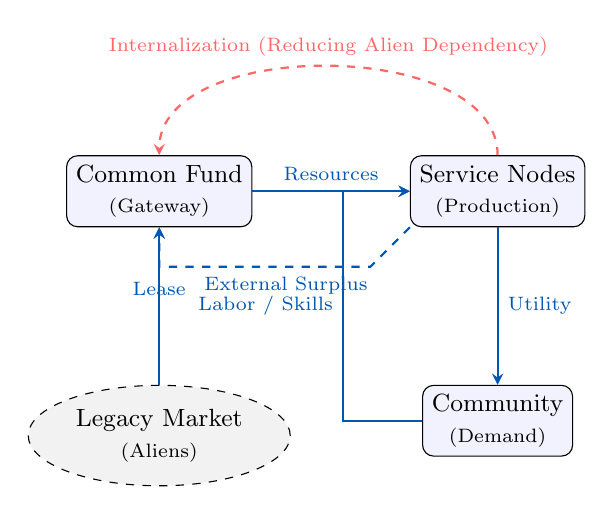
\begin{tikzpicture}[
        node distance = 2cm,
        auto,
        % Add 'align=center' to both styles below
        block/.style = {rectangle, draw, fill=blue!5, rounded corners, font=\headerfont\small, text centered, minimum width=1.5cm, minimum height=0.5cm, align=center},
        external/.style = {ellipse, draw, fill=gray!10, dashed, font=\headerfont\small, text centered, minimum width=1.5cm, align=center},
        arrow/.style = {->, >=stealth, thick, color=collectiveBlue}
    ]

    % Nodes
    \node [block] (fund) {Common Fund \\ \scriptsize (Gateway)};
    \node [external, below=of fund] (aliens) {Legacy Market \\ \scriptsize (Aliens)};
    \node [block, right=of fund] (nodes) {Service Nodes \\ \scriptsize (Production)};
    \node [block, below=of nodes] (demand) {Community \\ \scriptsize (Demand)};

    % Flows
    \draw [arrow] (aliens) -- node[above] {\scriptsize Lease} (fund);
    \draw [arrow] (fund) -- node[above] {\scriptsize Resources} (nodes);
    \draw [arrow] (nodes) -- node[right] {\scriptsize Utility} (demand);
    
    % The "Leaching" Loop
    \draw [arrow] (demand.west) -- ++(-1,0) |- node[pos=0.25, left] {\scriptsize Labor / Skills} (nodes.west);
    
    % Feedback to Fund (Decreasing over time)
    \draw [arrow, dashed] (nodes.south west) -- ++(-0.5,-0.5) -| node[pos=0.2, below] {\scriptsize External Surplus} (fund.south);

    % The "Obsolescence" Arrow
    \draw [arrow, color=red!60, dashed] (nodes.north) .. controls +(0,1.5) and +(0,1.5) .. node[above] {\scriptsize Internalization (Reducing Alien Dependency)} (fund.north);

    \end{tikzpicture}
    \caption{The Metabolic Leaching Strategy: Transitioning from External Lease to Internal Autonomy.}
\end{figure}



\section{Conclusion}

The architecture of \textbf{Collective} represents a departure from the historical view of the economy as a series of chaotic, zero-sum trades. By reconceptualizing resource allocation as a transparent, ubiquitous computational process, we address the systemic failures of information entropy, resource waste, and artificial scarcity that characterize the legacy market. 

Through the rigorous modeling of \textbf{Service Nodes} and the decoupling of lifestyle construction (Value) from social governance (Tokens), Collective creates a self-correcting metabolism. The system does not seek to overthrow the existing world through force, but to "leach" its utility—providing a superior, high-integrity alternative that naturally absorbs demand as its internal efficiency outpaces the speculative market.

The federated mesh of \textbf{Societies} and \textbf{Common Funds} provides the necessary legal and metabolic shielding for these bubbles of initiative to flourish. As these cells multiply and peer with one another, the dependence on legacy currency and external ownership asymptotically approaches zero. 

Ultimately, Collective is a protocol for human agency. It transforms the "invisible hand" of the market into an explicit, community-driven pulse. In this new paradigm, we move toward a future where the only investment is our labor, the only limit is our collective knowledge, and the primary output is the sustained flourishing of every member of the mesh. 

The transition is no longer a matter of political will, but of architectural implementation. The mesh is waiting to be booted.


\bibliographystyle{plain} % Or 'alpha', 'unsrt', etc.
\bibliography{references} % This assumes your file is named references.bib

\end{multicols}

\newpage

\section*{Appendix A: The Community Kitchen Reference Node}

To illustrate the practical application of the Service Node Modeler, we present the architecture of a "Nourishment Node." This node operates within a local Society to provide daily meals to Community Members while managing the "Leaching" of external food supplies.

\subsection*{A.1 Work Breakdown Structure (WBS)}
The Kitchen Node consists of three primary Task Classes imported from the Global \textbf{Body of Knowledge (BoK)}:
\begin{enumerate}
    \item \textbf{Preparation (Skill: Culinary.Level\_1):} The conversion of raw ingredients into utility.
    \item \textbf{Hospitality (Skill: Social.Mediation):} The management of the physical space and member interaction.
    \item \textbf{Stocking (Skill: Logistics.Basic):} The monitoring of inventory and triggering of procurement requests.
\end{enumerate}

\subsection*{A.2 Interaction with the Common Fund}
The Kitchen utilizes a "Hybrid Sourcing" logic. High-perishables (leafy greens, eggs) are sourced from an internal \textit{Agricultural Node} via "Direct Consumption" tasks. Bulk staples (grains, oils) not yet internalized are leased via the \textbf{Common Fund}. 

When the Stocking Task identifies a grain level below the 20\% threshold, the Node Modeler automatically issues a "Lease Request" to the Common Fund. The Fund pays the "Alien" supplier in legacy currency, and the Kitchen Node escalates a "Receiving" task to the local Worker pool.

\subsection*{A.3 Governance and Token Weighting}
In this specific node, the "Head Chef" role is not a permanent title but a state granted to the Member with the highest \textit{Nourishment Tokens}. 
\begin{itemize}
    \item \textbf{Value Payment:} Due to the high demand for dinner services, the "Preparation" tasks between 18:00 and 20:00 carry a $1.5\times$ Value weight.
    \item \textbf{Spend-to-Change:} A Member wishing to change the menu (altering the Resource Requirements in the WBS) must stake 50 Tokens. If the new menu results in excessive waste (Resource Leakage), those tokens are depleted.
\end{itemize}

\begin{figure*}[h]
\centering
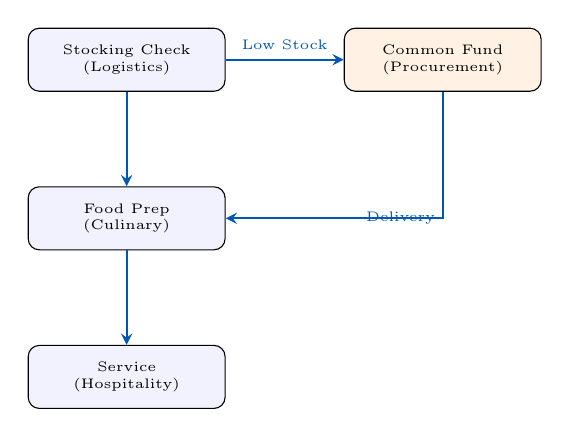
\begin{tikzpicture}[
    node distance = 1.2cm,
    align=center,
    block/.style = {rectangle, draw, fill=blue!5, rounded corners, font=\tiny, minimum width=2.5cm, minimum height=0.8cm},
    arrow/.style = {->, >=stealth, thick, color=collectiveBlue}
]
    % Sequence Flow
    \node [block] (inventory) {Stocking Check \\ (Logistics)};
    \node [block, below=of inventory] (prep) {Food Prep \\ (Culinary)};
    \node [block, below=of prep] (serve) {Service \\ (Hospitality)};
    \node [block, right=1.5cm of inventory, fill=orange!10] (fund) {Common Fund \\ (Procurement)};

    % Connections
    \draw [arrow] (inventory) -- (prep);
    \draw [arrow] (prep) -- (serve);
    \draw [arrow] (inventory) -- node[above, font=\tiny] {Low Stock} (fund);
    \draw [arrow] (fund) |- node[pos=0.7, right, font=\tiny] {Delivery} (prep);
\end{tikzpicture}
\caption{Simplified BPMN logic for a Nourishment Service Node.}
\end{figure*}

\newpage
\section*{Appendix B: Lexicon of the Collective}

\begin{description}[style=nextline, leftmargin=1em, font=\bfseries\headerfont\color{collectiveBlue}]
    \item[Aliens] The conceptual label for external market entities and legacy systems operating on capital-driven logic.
    \item[Availability Task] A scheduled task that compensates Workers for being in a "ready-to-serve" state to solve the cold-start problem for on-demand services.
    \item[Body of Knowledge (BoK)] A specialized Digital Society that maintains the global registry of Task definitions and verifies Member skill competencies.
    \item[Leaching] The strategic process of incrementally internalizing production to reduce and eventually eliminate dependency on legacy currency and external leases.
    \item[Service Node] The primary unit of production within the mesh; a recursive, self-governing entity defined by a Work Breakdown Structure (WBS).
    \item[Society] A specialized node governing the legal and territorial logic of a community instance, managing the physical "Right to Inhabit."
    \item[Unbounded Negative Balance] A feature of the Value system allowing Members to consume resources based on potential or need without punitive interest, signaled as an investment in the Member’s future labor.
\end{description}

\newpage
\section*{Appendix C: Service Designer’s Quick-Start}

To instantiate a new Service Node within an existing Society, a Designer must follow the "Instantiation Protocol":

\begin{enumerate}
    \item \textbf{Identify Latent Demand:} Use the local \textit{Prospecting Engine} to verify that a community need is currently unmet (e.g., a gap in local renewable energy maintenance).
    \item \textbf{Draft the WBS:} In the Modeler, drag and drop standardized \textit{Task Blocks} from the relevant BoK. 
    \item \textbf{Define Environment Properties:} Set the "Trigger Events" (e.g., \textit{If Grid\_Voltage < 210V, trigger Maintenance\_Task}).
    \item \textbf{Determine Resource Mapping:} Categorize every required input as either \textit{Internal} (sourced from the Mesh) or \textit{External} (requiring a Common Fund lease).
    \item \textbf{Ratification:} Present the model to the local Society. Stake the required \textit{Reputation Tokens} to commit the WBS to the local ledger.
\end{enumerate}



\noindent \textit{Note: Designers are encouraged to "Fork" existing high-efficiency Node models from the Global BoK to accelerate community bootstrapping.}


\end{document}